\ProvidesFile{definitions.tex}[Определения]
\newpage
\section{Определения}
\subsection{Понятие стереографической проекции}
\begin{definition}
    Расширенной комплексной плоскостью $\overline{\C}$ называется одноточечная компактификация $\C$, получаемая добавлением к $\C$ новой точки $\infty$. База окрестностей точки $\infty$ на $\overline{\C}:=\C\cup \left\{\infty\right\}$ задаётся внешностями кругов $\left\{z\in\C\colon |z|>R\right\}\cup \left\{\infty\right\}$. 
\end{definition}

Пусть $S:= \left\{(\xi,\eta,\zeta)\in\R^3\colon \xi^2+\eta^2+(\zeta-\frac{1}{2})^2=\frac{1}{4}\right\}$ - сфера в евклидовом пространстве $\R^3$ с центром в точке $(0,0,\frac{1}{2})$ радиуса $\frac{1}{2}$. 

\begin{center}
  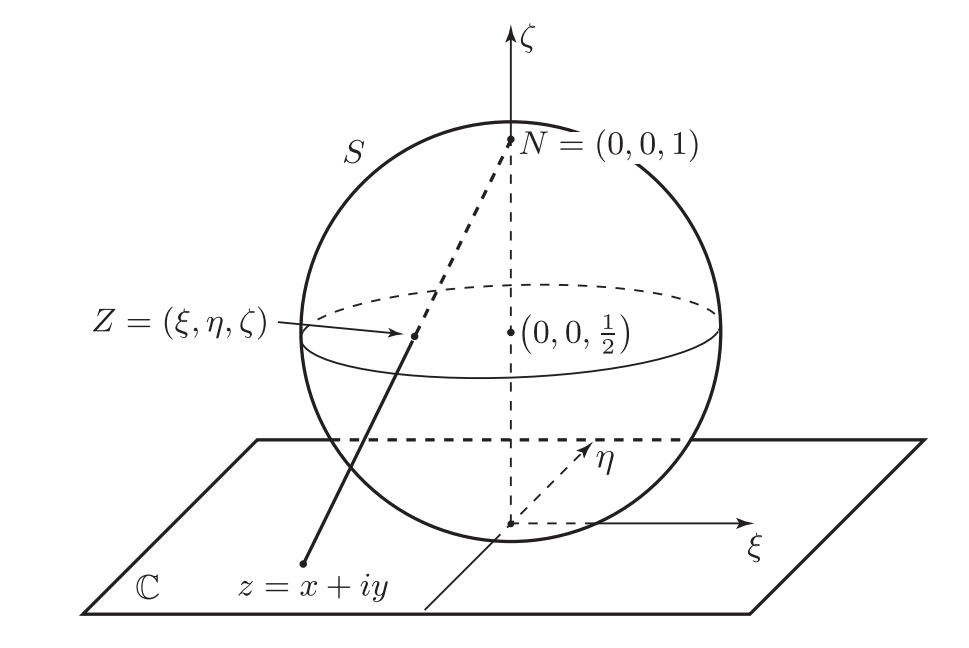
\includegraphics[scale=0.6]{1.png}
\end{center}

Отождествим комплексную плоскость $\C$ с плоскостью $\left\{\zeta=0\right\}$ в $\R^3$ и сопоставим каждой точке $z=x+iy$ точку $Z=(\xi,\eta,\zeta)$ пересечения сферы $S$ лучом, соединяющим $z$ с северным полюсом $N=(0,0,1)$ сферы $S$. Для того чтобы выразить координаты точки $Z$ через $z$, запишем луч параметрически в виде
\[\xi=tx,\q \eta = ty,\q \zeta = 1-t\]
Его точка пересечения со сферой $S$ отвечает значению параметра $t$, которое находится из уравнения
\[t^2(x^2+y^2) + \left(\frac{1}{2}-t\right)^2=\frac{1}{4}\]
\[t^2|z|^2+t^2 - t +\frac{1}{4}=\frac{1}{4}\]
\[t^2(1+|z|^2)=t,\q t\neq0\]
\[\implies t = \frac{1}{1+|z|^2}\]
Следовательно, координаты искомой точки $Z=(\xi,\eta,\zeta)$ вычисляются по формуле
\[\xi = \frac{x}{1+|z|^2},\q \eta = \frac{y}{1+|z|^2},\q \zeta = \frac{|z|^2}{1+|z|^2}\]
Обратное отображение находится из соотношения $t=1-\zeta$, откуда
\[x=\frac{\xi}{1-\zeta},\q y=\frac{\eta}{1-\zeta}\]

Из приведённых формул следует, что стереографическая проекция $Z\leftrightarrow z$ устанавливает взаимно однозначное соответствие между точками сферы $S\setminus \left\{N\right\}$ без северного полюса $N$  и комплексной плоскости $\C$. Более того, при этом отображении базе проколотых окрестностей точки $\infty \in \overline{\C}$, состоящей из внешностей кругов $\{z\in\C\colon |z| > R\}$, будет отвечать база проколотых окрестностей северного полюса $N$ на сфере $S$. Таким образом, если продлить стереографическую проекцию $S\setminus \left\{N\right\}\leftrightarrow \C$ до соответствия $S\leftrightarrow \overline{\C}$, сопоставляя северному полюсу $N$ точку $\infty \in \overline{\C}$, то полученное отображение будет осуществлять гомеоморфизм сферы $S$ с расширенной комплексной плоскостью $\overline{\C}$.

Построенная модель расширенной комплексной плоскости $\C$ называется сферой Римана.
\subsection{Сходимость последовательности в расширенной комплексной плоскости}
\begin{definition}
  \begin{enumerate}
    \item Метрика на $\C$:
    \[\rho(z_1,z_2) = |z_1-z_2|\]
    \item Сферическая метрика на $\C$:
    \[\rho_{\text{сф}}(z_1,z_2)=|Z_1-Z_2|\]
  \end{enumerate}
\end{definition}
\begin{definition}
  $z_n\to \infty$, если $|z_n|\to+\infty$
\end{definition}
\begin{theorem}
  Сходимость в $\overline{\C}$ по $\rho$ и по $\rho_{\text{сф}}$ эквивалентны.
\end{theorem}
\subsection{$\C$-дифференцируемость в расширенной комплексной плоскости}
\begin{definition}
  Функция $f\colon U(z_0)\to\C$ $\C$-дифференцируема в т. $z_0$, если $\exists a\in\C\colon$
  \[f(z) - f(z_0) = a\Delta z + \overline{o}(\Delta z),\q\Delta z\to 0\]
  Т.е. $\exists \Lim{z}{z_0}\frac{f(z)-f(z_0)}{z-z_0}=:f'(z_0)\in\C$
\end{definition}
\begin{definition}
  $f\colon U(\infty)\to \C$, т.е. $f(\infty)\in\C$. Тогда $f$ $\C$-дифференцируема в $\infty$, если $g(z):=f(\frac{1}{z})$ (где $\frac{1}{z}\colon 0\to \infty,\q \infty\to 0$) $\C$-дифференцируема в 0.  
\end{definition}
\begin{definition}
  $f\colon U(z_0)\to \overline{\C}$ и $f(z_0)=\infty$. Тогда $f$ $\C$-дифференцируема в $z_0$, если $g(z):=\frac{1}{f(z)}$ $\C$-дифференцируема в $z_0$.  
\end{definition}
\begin{definition}
  $f\colon U(\infty)\to \overline{\C}$ и $f(\infty)=\infty$ . Тогда $f$ $\C$-дифференцируема в $\infty$, если $g(z):=\frac{1}{f(\frac{1}{z})}$  $\C$-дифференцируема в 0.  
\end{definition}
\subsection{Условие Коши-Римана}
\begin{theorem}
  $f\in U(z_0)\to\C$, $f$ $\C$-дифференцируема в т. $z_0$ $\lra$ $f$ $\R$-дифференцируема и выполнено условие Коши-Римана:
  \[ 
  \begin{cases}
    u'_x = v'_y, \\
    u'_y=-v'_x, 
  \end{cases}\lra \p{f}{\overline{z}}(z_0)=0\]
\end{theorem}
\subsection{Голоморфность функции в точке расширенной комплексной плоскости}
\begin{definition}
  $f$ голоморфна в т. $z_0$, если она $\C$-дифференцируема в некоторой окрестности $U(z_0)$. Обозначение: $f\in\O(z_0)$
\end{definition}
На точки $\overline{\C}$ голоморфность распространяется также, как и $\C$-дифференцируемость. 
\subsection{Конформность отображения в точке расширенной комплексной плоскости}
\begin{definition}
  $f\colon U(z_0)\to\C$ конформна в т. $z_0$, если $f\in \O(z_0)$ и $f'(z_0)\neq 0$. 
\end{definition}
На точки $\overline{\C}$ конформность распространяется также, как и $\C$-дифференцируемость.
\subsection{Конформность отображения в области}
\begin{definition}
  $f\colon D\to\overline{\C}$ конформна в области $D\subseteq \overline{\C}$, если $f$ конформна в каждой т. $D$ и инъективна (однолистна) в $D$.
\end{definition}
\subsection{Теорема об отображении границы области под действием отображения, конформного в этой
области}
\begin{theorem}
  $f\in C(\overline{D})$ и $f$ конформна в $D$. $\gamma:=\partial D$ и $f(\gamma)=\widetilde{\gamma}$ - граница, которая задаёт область $\widetilde{D}$ с учётом обхода. Тогда $f(D)=\widetilde{D}$. 
\end{theorem}
\subsection{Сохранение углов между кривыми под действием конформного отображения}
\begin{theorem}
  $f$ конформна в $z_0$; $\gamma_1,\gamma_2$ - гладкие кривые $\colon\q z_0\in \gamma_1,\gamma_2$. Тогда $\widetilde{\gamma_1}:=f(\gamma_1),\q \widetilde{\gamma_2}:=f(\gamma_2)$ - гладкие кривые, причём $\angle(\gamma_1,\gamma_2)|_{z_0} = \angle(\widetilde{\gamma_1},\widetilde{\gamma_2})|_{z_0}$ 
\end{theorem}
\subsection{Круговое свойство ДЛО}
\begin{theorem}
  ДЛО переводит обобщённую окружность в обобщённую окружность.
\end{theorem}
\subsection{Свойство симметрии для ДЛО}
\begin{theorem}
  Пусть $\g$ - обобщённая окружность, $z_1,\q z_2$ - симметричны относительно неё и $w$ - ДЛО. Тогда $w_1:=w(z_1),\q w_2:=w(z_2)$ - симметричны относительно $w(\g)$ 
\end{theorem}
\subsection{Правило трех точек для ДЛО}
\begin{theorem}
  $z_1,z_2,z_3\in\RC$ и $w_1,w_2,w_3\in\RC$. Тогда $\exists!\q w=f(z)$ - ДЛО : $w_k=f(z_k)$ 
\end{theorem}
\subsection{Интеграл комплекснозначной функции вдоль гладкого пути}
\begin{definition}
  Пусть $\g$ - гладкий путь, $f\colon\C\to\C,\q f=u+iv$. Тогда
  \[\int_{\g}f(z)\d z:=\int_{0}^{1}f(\g(t))\cdot \g(t)'\d t=\int_{0}^{1}(ux'-vy')(t)\d t + i \int_{0}^{1}(vx' + uy')(t)\d t\]
  Если $\g$ - параметризация кривой $\gamma$ и задано направление обхода $\gamma$, то
  \[\int_{\gamma}f(z)\d z := \int_{\g}f(z)\d z\]
\end{definition}
\subsection{Свойства интеграла вдоль пути}
Свойства:
\begin{enumerate}
  \item Линейность
  \item Независимость от параметризации (следует из замены переменной)
  \item Зависит от направления, т.е.
  \[\int_{\gamma^+}f(z)\d z = - \int_{\gamma^-}f(z)\d z\]
  \item Аддитивность: $\gamma = \gamma_1\cup \gamma_2$
  \[\int_{\gamma}f(z)\d z = \int_{\gamma_1}f(z)\d z + \int_{\gamma_2}f(z)\d z\]
  \item Верны неравенства 
  \[\left|\int_{\gamma}f(z)\d z\right|\leqslant \int_{0}^{1}\left|f(\g(t))\g(t)'\right|\d t\leqslant M \int_{0}^{1}\left|\g(t)'\right|\d t= M |\gamma|\]
  где $M$ из первой теоремы о среднем. 
\end{enumerate}
\subsection{Лемма Гурса}
\begin{theorem}
  Пусть $f\in\O(D)$. Тогда $\forall \Delta\colon \overline{\de} \in D$ выполнено:
  \[\oint\limits_{\partial\de}f(z)\d z=0\]
\end{theorem}
\subsection{Первообразная в области}
\begin{definition}
  Первообразной $f$ в области $D$ называется $F\in\O(D)\colon F'=f$.
\end{definition}
\subsection{Теорема о существовании первообразной в круге}
\begin{theorem}
  $f\in C(D)$ и $\forall \overline{\de}\in D\q \oint\limits_{\partial\de}f(z)\d z=0$, где $D=\left\{|z-a|<R\right\}$. Тогда $\exists F$ - первообразная $f$ в $D$. 
\end{theorem}
\subsection{Первообразная вдоль пути}
\begin{definition}
  $f\in C(D)$, $\g$ - путь $\colon [0,1]\to D$. Тогда $\Phi\colon [0,1]\to\C$ называется первообразной $f$ вдоль пути $\g$, если
  \begin{enumerate}
    \item $\Phi\in C([0,1])$
    \item $\forall t_0\in[0,1]\q\exists U_\delta(t_0)\subset [0,1],\q\exists U_\e(z_0)\subset D$  (где $z_0=\g(t_0)$) такие, что $\exists F_\e$ - первообразная $f$ в $U_\e(z_0)\colon \Phi(t) = F_\e(\g(t))\q\forall t\in U_\delta(t_0)$. 
  \end{enumerate}
\end{definition}
\subsection{Теорема о существовании первообразной вдоль пути}
\begin{theorem}
  $f\in\O(D),\q \g\colon[0,1]\to D$ - путь. Тогда $\exists$ первообразная вдоль пути $\Phi(t)$ и любые две из первообразных отличаются на константу. 
\end{theorem}
\subsection{Формула Ньютона-Лейбница для голоморфной функции}
\begin{theorem}
  $f\in\O(D),\q \g\colon [0,1]\to D$, $\Phi$  - первообразная вдоль пути $\g$. Тогда
  \[\int_{\g}f(z)\d z = \Phi(1) - \Phi(0)\]
\end{theorem}
\subsection{Гомотопные пути}
\begin{definition}
  $\g_0,\g_1\colon [0,1]\to D,\q \g_0(0)=\g_1(0)=:a$ и $\g_0(1) = \g_1(1) =: b$.

  Тогда $\g_0$ гомотопен $\g_1$ в $D$, если $\exists\g\colon[0,1]^2\to D\colon \g\in C([0,1]^2)$ и $\g(0,t)=\g_0(t),\q \g(1,t)=\g_1(t)$ и $\forall s \in [0,1]$:
  \[ 
  \begin{cases}
    \g(s,0)=a\\
    \g(s,1)=b\\
  \end{cases}\]
  \begin{center}
  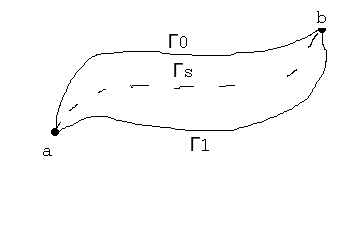
\includegraphics{4.png}
  \end{center}

  Обозначение: $\g_0\sim\g_1$
\end{definition}
\begin{definition}
  Замкнутые пути $\g_0,\g_1\colon [0,1]\to D$ называют гомотопными, если $\exists\g\colon[0,1]^2\to D\colon \g\in C([0,1]^2)$ и $\g(0,t)=\g_0(t),\q \g(1,t)=\g_1(t)$ и $\forall s \in [0,1]$ $\g(s,0)=\g(s,1)$. 

  Замкнутый путь гомотопен 0 $(\g\sim0)$, если он гомотопен постоянному пути $\g_1\equiv const$, т.е. если можно сжать путь в точку.
\end{definition}
\subsection{Теорема о гомотопии (об интегралах вдоль гомотопных путей)}
\begin{theorem}
  $f\in\O(D)$ и $\g_0\sim\g_1$ в $D$. Тогда
  \[\int_{\g_1}f(z)\d z=\int_{\g_2}f(z)\d z\]
\end{theorem}
\subsection{Интегральная теорема Коши для односвязной области}
\begin{theorem}
  $D$ - односвязная область, $f\in\O(D)$, $\g\colon[0,1]\to D$ - замкнутый путь. Тогда
  \[\oint\limits_{\g}f(z)\d z=0\]
\end{theorem}
\subsection{Теорема о существовании первообразной в односвязной области}
\begin{theorem}
  $D$ - односвязная область, $f\in\O(D)$. Тогда $\exists F$ - первообразная $f$ в $D$. 
\end{theorem}
\subsection{Критерий существования первообразной в произвольной области}
\begin{theorem}
  Если $f\in\O(D)$ и $\oint\limits_{\g}f(z)\d z = 0$ $\forall\g$ - замкнутого пути, то $\exists F$ - первообразная $f$ в $D$. 

\end{theorem}
\subsection{Интегральная теорема Коши для многосвязной области}
\begin{theorem}
  $f\in\O(G)$, $\overline{D}\subset G$ и $\partial D$ - простая кривая, т.е. $\partial D=\gamma_0\cup\dots\cup\gamma_n$, где $\gamma_i$ - простые и кусочно-гладкие попарно непересекающиеся кривые, где $\gamma_0$ - внешняя граница, а $\gamma_1,\dots,\gamma_n$ - внутренние. Тогда
  \[\int_{\partial D^+}f(z)\d z = 0\]
  где
  \[\int_{\partial D^+}f(z)\d z = \int_{\gamma_0^+}f(z)\d z - \Sum{i=1}{n}\int_{\gamma_i^+}f(z)\d z\]
\end{theorem}
\subsection{Интегральная формула Коши}
\begin{theorem}
  $f\in\O(G),\q \overline{D}\subset G,\q \partial D$ - простая. Тогда $\forall z\in D$
  \[f(z) = \frac{1}{2\pi i} \oint\limits_{\partial D^+}\frac{f(\zeta)}{\zeta - z}\d \zeta\]
\end{theorem}
\subsection{Теорема об интеграле вдоль пути от равномерно сходящейся последовательности функций}
\begin{theorem}
  $f_n\overset{\gamma}{\rightrightarrows}f$ и $\gamma$ - гладкая кривая, $f_n\in C(\gamma)$. Тогда
  \[\int_{\gamma}f_n(z)\d z\underset{n\to \infty}{\to} \int_{\gamma}f(z)\d z\]
\end{theorem}
\subsection{Теорема Тейлора для голоморфных функций (о разложимости голоморфной функции в ряд
Тейлора)}
\begin{theorem}
  $f\in\O(D)$ и $U_R(a)\subset D$. Обозначим:
  \[c_n:= \frac{1}{2\pi i} \oint\limits_{|z-a|=r}\frac{f(\zeta)}{(\zeta-a)^{n+1}}\d \zeta\text{, где $0<r<R,\q n\in\N_0$}\]
  Тогда числа $c_n$ не зависят от выбора числа $r$, ряд $\Sum{n=0}{+\infty}c_n(z-a)^n$ сходится в $U_R(a)$, причём к $f(z)$, т.е. $\forall z\in U_R(a)$
  \[f(z) = \Sum{n=0}{+\infty}c_n(z-a)^n\]
  Числа $c_n$ называются коэффициентами Тейлора функции $f$ в точке $a$, а ряд - рядом Тейлора функции $f$ в точке $a$.
\end{theorem}
\subsection{Неравенство Коши для коэффициентов Тейлора}
\begin{theorem}
  В условиях теоремы Тейлора
  \[|c_n|\leqslant \frac{M(r)}{r^n}\text{, где $M(r):=\Sup{|z-a|=r}|f(z)|$}\]
\end{theorem}
\subsection{Целая функция}
\begin{definition}
  Функцию $f$ называют целой, если $f\in\O(\C)$ 
\end{definition}
\subsection{Теорема Лиувилля}
\begin{theorem}
  $f\in\O(\C)$ и $f\in{\rm B}(\C)$. Тогда $f\equiv const$.
\end{theorem}
\subsection{Формула Коши-Адамара (для радиуса сходимости) и теорема Коши-Адамара}
\begin{theorem}
  Пусть дан степенной ряд $\Sum{n=0}{+\infty}b_n(z-a)^n$, $L:=\uplim{n}{\infty}\sqrt[n]{|b_n|}$. Положим
  \[R:= 
  \begin{cases}
    \infty, &L=0\\
    0, &L=\infty\\
    \frac{1}{L}, &\text{иначе }\\
  \end{cases}\]
  \begin{enumerate}
    \item Если $R=0$, то ряд сходится в $z=a$ и расходится в $\C\setminus \left\{a\right\}$ 
    \item Если $R=\infty$, то ряд сходится в $\forall z\in\C$ 
    \item Если $R\neq 0,\infty$, то ряд сходится в $U_R(a)$ и расходится при $z\colon |z-a|>R$. 
  \end{enumerate}

  (нестрогая) Формула Коши-Адамара:
  \[\frac{1}{R} = \uplim{n}{\infty}\sqrt[n]{|b_n|}\]
\end{theorem}
\subsection{Теорема Абеля (о равномерной сходимости на компакте внутри круга сходимости степенного
ряда)}
\begin{theorem}
  Пусть дан степенной ряд $\Sum{n=0}{+\infty}b_n(z-a)^n$, $R$ - его радиус сходимости. Тогда $\forall K$ - компакта $\subset U_R(a)$ ряд сходится на $K$ равномерно.
\end{theorem}
\subsection{Теорема о голоморфности суммы степенного ряда}
\begin{theorem}[(О голоморфности суммы степенного ряда)]
  $f(z):=\Sum{n=0}{+\infty}b_n(z-a)^n$, $R$ - радиус сходимости. Тогда $f\in\O(U_R(a))$ и $f'(z)=\Sum{n=1}{+\infty}b_n\cdot n(z-a)^{n-1}$ 
\end{theorem}
\subsection{О бесконечной дифференцируемости голоморфной функции}
\begin{theorem}
  $f\in\O(D)$. Тогда $\forall n\in\N\q f^{(n)}\in \O(D)$, причём если $f(z):=\Sum{n=0}{+\infty}c_n(z-a)^n$, то $f^{(k)}(z)=\Sum{n=k}{+\infty}c_n \frac{n!}{(n-k)!}(z-a)^{n-k}$ 
\end{theorem}
\subsection{Связь коэффициентов Тейлора и производных голоморфной функции}
\begin{theorem}
  Коэффициэнты Тейлора могут быть выражены как $c_n=\frac{f^{(n)}(a)}{n!}$
\end{theorem}
\subsection{Интегральная формула Коши для производных голоморфной функции}
\begin{theorem}
  $f\in\O(G),\q \overline{D}\subset G$ и $\partial D$ состоит из конечного числа простых замкнутых кривых. Тогда
  \[f^{(n)}(z)=\frac{n!}{2\pi i} \oint\limits_{\partial D^+}\frac{f(\zeta)}{(\zeta - z)^{n+1}}\d \zeta\]
\end{theorem}
\subsection{Теорема Мореры}
\begin{theorem}
  Пусть $f$ в $D$ удовлетворяет условию треугольника, т.е. $f\in C(D)$ и $\forall \overline{\Delta}\subset D\q \oint\limits_{\partial \Delta}f(z)\d z=0$. Тогда $f\in\O(D)$. 
\end{theorem}
\subsection{Три эквивалентных определения голоморфной функции}
\begin{theorem}
  $f$ голоморфна в т. $a$ эквивалентно любому из следующих условий: 
  \begin{enumerate}
    \item $f$ $\C$-дифференцируемо в $U(a)$
    \item В некоторой $U(a)$ $f(z)=\Sum{n=0}{+\infty}c_n(z-a)^n\q\forall z\in U(a)$ 
    \item В некоторой $U(a)$ выполняется условие треугольника, т.е. $f\in C(U(a))$ и \[\forall\overline{\Delta}\subset U(a)\q \oint\limits_{\partial \Delta}f(z)\d z=0\] 
  \end{enumerate}
\end{theorem}
\subsection{Теорема о представлении голоморфной функции в окрестности нуля}
\begin{theorem}
  $f\in\O(U(a))$ и $f(a)=0$. Тогда либо $\exists \delta>0\colon f\equiv 0$ в $U_\delta(a)$, либо $\exists \delta>0\colon f(z)=(z-a)^Ng(z)$, где $g\in\O(U_\delta(a))$ и $g(a)\neq0$. 
\end{theorem}
\subsection{Порядок нуля голоморфной функции}
\begin{definition}
  Пусть $f\in\O(U(a)),\q f(a)=0$ и $\nexists\delta>0\colon f(z)\equiv 0$ в $U_\delta(a)$. Тогда число $N\colon f(z)=(z-a)^Ng(z)$, где $g(a)\neq 0,\q g\in\O(U_\delta(a))$ называют порядком нуля $f$ в точке $a$, т.е.
  \[N=\min \left\{n\colon c_n\neq 0\right\} = \min \left\{n\colon f^{(n)}(a)\neq 0\right\}\]
  Если можно доопределить $f(\infty)=0$ по непрерывности и $f\in\O(\infty)$, то порядком 0 в $\infty$ называется порядок 0 у $g(z):=f(\frac{1}{z})$ в 0. 
\end{definition}
\subsection{Теорема об изолированности нулей голоморфной функции}
\begin{theorem}
  $f\in\O(U(a))$ и $f(a)=0$. Тогда либо $f\equiv 0$ в $U_\delta(a)$, либо $\exists\delta>0\colon f(z)\neq 0$ в $\overset{\circ}{U}_\delta(a)$. 
\end{theorem}
\subsection{Теорема единственности для голоморфных функций}
\begin{theorem}
  $f,g\in\O(D),\q E\subset D$, $E$ - множество с предельной точкой в $D$ и $f = g$ в $E$. Тогда $f=g$ в $D$. 
\end{theorem} 
\subsection{Теорема Вейерштрасса}
\begin{theorem}
  Пусть $f_n\in\O(D)$ и $\forall K\subset D$ - компакта $f_n\overset{K}{\rightrightarrows}f$. Тогда
  \begin{enumerate}
    \item $f\in \O(D)$
    \item $f^{(k)}(z)=\Lim{n}{\infty}f_n^{(k)}(z)$
    \item $f_n^{(k)}\overset{K}{\rightrightarrows}f^{(k)}\q\forall K$ 
  \end{enumerate}
\end{theorem}
\subsection{Теорема Рунге}
\begin{theorem}
  $D$ - односвязная область, $f\in\O(D)$. Тогда $\exists R_n(z)\colon R_n(z)\overset{K}{\rightrightarrows}f(z)\q\forall K\subset D$ - компакта, где $R_n$ - рациональные функции, т.е. $R_n(z)=\frac{P_n(z)}{Q_n(z)}$, где $P_n,Q_n$ - многочлены. 
\end{theorem}
